\documentclass[12pt]{article}
\usepackage[a4paper, total={6in, 9in}]{geometry}
\usepackage{amsmath, amssymb}
\usepackage{graphicx}
\usepackage{enumitem}
\usepackage{fancyvrb}
\usepackage[skip=\medskipamount]{parskip}
\usepackage{pdfpages}
\usepackage{array}
\usepackage{tabularray}
\usepackage{longtable}
\usepackage{tikz}
\usepackage{float}
\setlength{\parindent}{0pt}

% \renewcommand*{\thesubsection}{\alph{subsection}}
% \renewcommand*{\theenumi}{\alph{enumi}}

\title{\vspace{-1.5cm}E0 259 Assignment-3}
\author{Aditya Gupta \\
SR No: 22205}
\date{}

\begin{document}
\maketitle

In this module, we have to study the effects of smoking on males and females. To do this, we use the data of the measurements of 41092 probes from 48 patients. The patients are divided equally into four groups: male smokers, male non-smokers, female smokers and female non-smokers. We will use a 2 way ANOVA test to determine the genes which are affected the most by smoking in males and females.

\section*{Data Preprocessing}
The data is given to us in a text format. We first convert it to a pandas dataframe for easier manipulation. Apart from the values of the probes for the different patients, we also have some columns with other information about the probe. One of these columns is labelled 'Go' which is not relevant to our analysis, and thus we drop this column. Then we also drop columns which have missing values in them. After this, we are left with 31502 probes and 48 patients. 

\section*{ANOVA Test}
Now we perform a 2 way ANOVA test on each of the remaining probes. To calculate the F statistic for each row, we use the following formula:
\begin{equation*}
    F = \frac{1/(rank(D) - rank(N))}{1/(n - rank(D))} \times \left( \frac{X^T(I - N(N^T N)^{\dagger}N^T)X}{X^T(I - D(D^T D)^{\dagger}D^T)X} - 1 \right)
\end{equation*}

where $n$ is the total number of patients and:

\[
D = \begin{bmatrix}
    1 & 0 & 0 & 0 \\
    \vdots & \vdots & \vdots & \vdots \\
    0 & 1 & 0 & 0 \\
    \vdots & \vdots & \vdots & \vdots \\
    0 & 0 & 1 & 0 \\
    \vdots & \vdots & \vdots & \vdots \\
    0 & 0 & 0 & 1 \\
    \vdots & \vdots & \vdots & \vdots \\
\end{bmatrix}_{48 \times 4} \quad
N = \begin{bmatrix}
    1 & 0 & 1 & 0 \\
    \vdots & \vdots & \vdots & \vdots \\
    1 & 0 & 0 & 1 \\
    \vdots & \vdots & \vdots & \vdots \\
    0 & 1 & 1 & 0 \\
    \vdots & \vdots & \vdots & \vdots \\
    0 & 1 & 0 & 1 \\
    \vdots & \vdots & \vdots & \vdots \\
\end{bmatrix}_{48 \times 4}
\]

Using this, we calculate the F statistic for each row. Then we calculate the p-value for each row using the F statistic with the help of scipy's stats module. To visualise the distribution of the p-values, we plot a histogram of the p-values for all the probes, with 100 bins.

\begin{figure}[h]
    \centering
    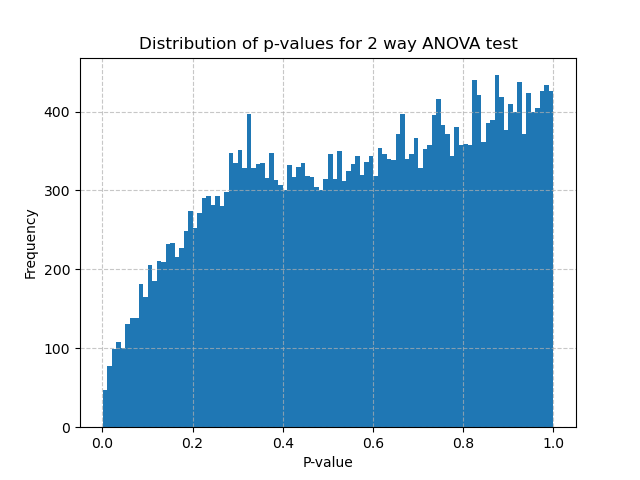
\includegraphics[width=0.8\textwidth]{output/p_values.png}
    \caption{Histogram of p-values for all probes}
\end{figure}

We can see that the distribution here is not uniform. Hence the null hypothesis that the gene expression is not affected by smoking is not true for all the probes. We can see a lot of probes with p-values less than 0.05, which means that the gene expression is affected by smoking for these probes. These probes can be used to study the effects of smoking on males and females.

\end{document}